\section{Creating a Simple Circuit}

We'll start with a very simple circuit. Let's build the circuit first, then we'll take a look at how it works afterwards.

	\begin{aside}[Solderless Breadboards]
		
		A common tool for building small electrical circuits is the \textit{solderless breadboard}.
		
		The breadboard consists of rows of square sockets, in which electrical components can be easily placed, with metal wire `lanes' running underneath the breadboard to make electrical connections.
			
		\begin{center}
			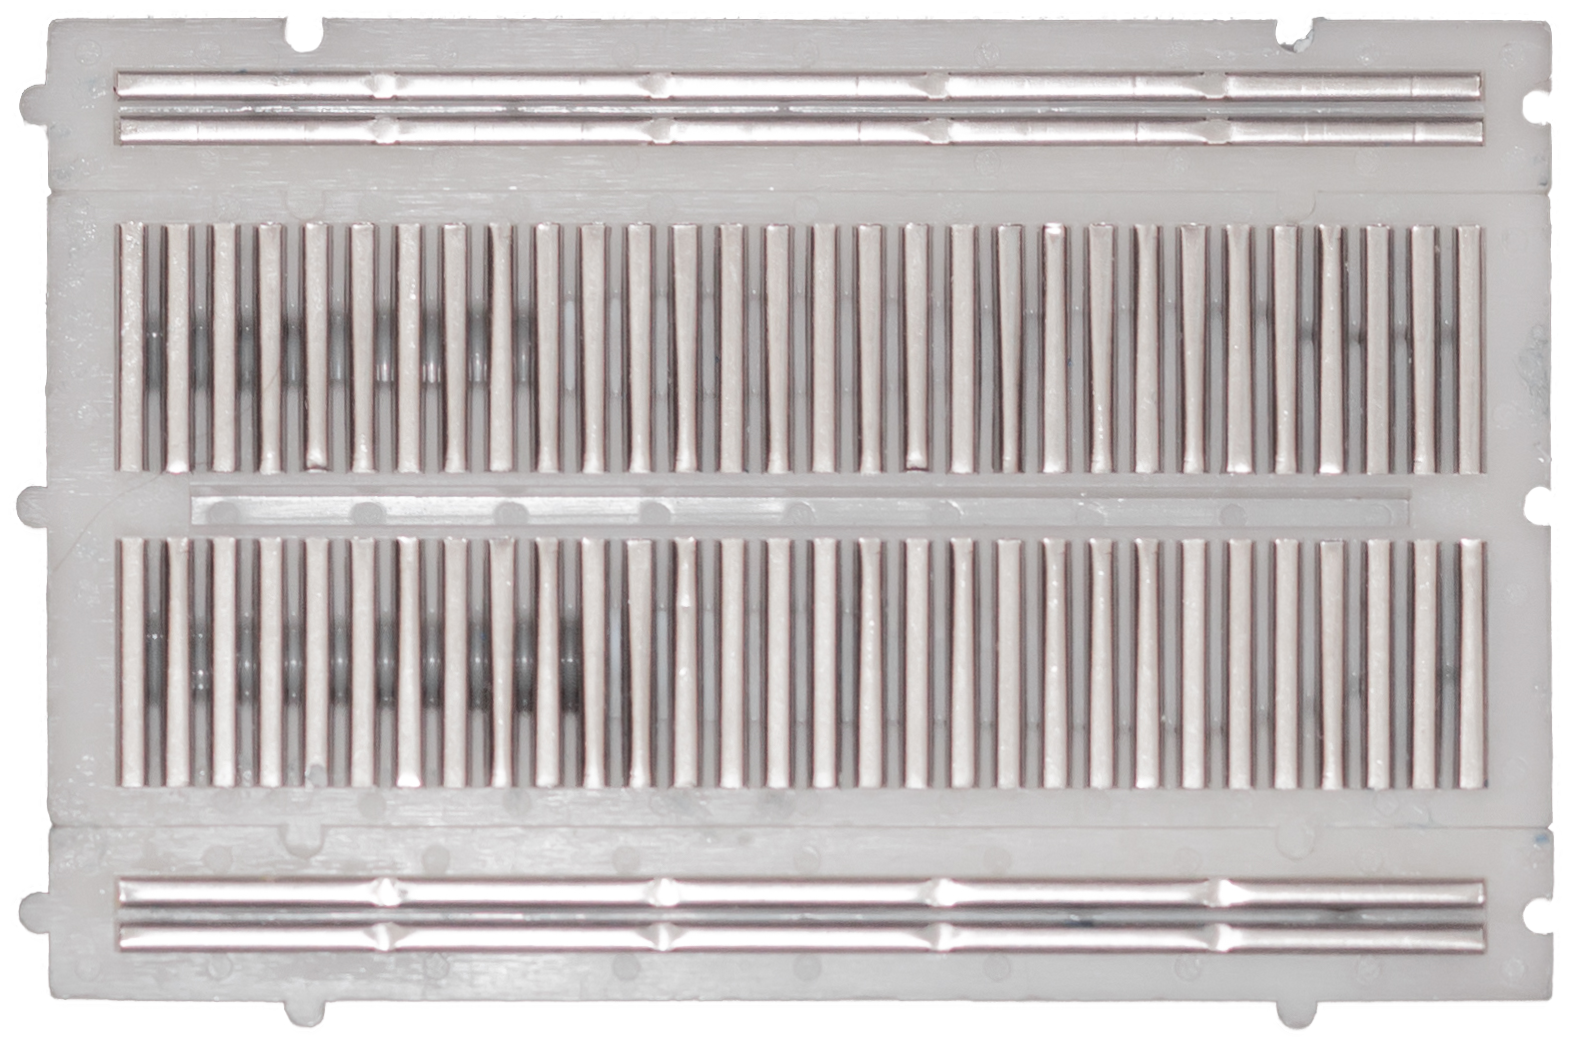
\includegraphics[width=0.7\linewidth]{McrRaspJam/011_Motors/1_LED/breadboard_underside}
		\end{center}
	
		The layout of `lanes' under a standard breadboard is shown above. Components need to be carefully placed to ensure a full circuit is made.
	
	\end{aside}


	Take your breadboard, and place it next to your Raspberry Pi. Then, take a red LED and place it across the central gap in your breadboard, as shown. (The longer lead of the LED should be on the side nearest your Raspberry Pi)
	
	Then, connect the positive side of the LED to the positive power rail on the breadboard using a male-to-male jumper cable, as shown.
	
	\begin{center}
		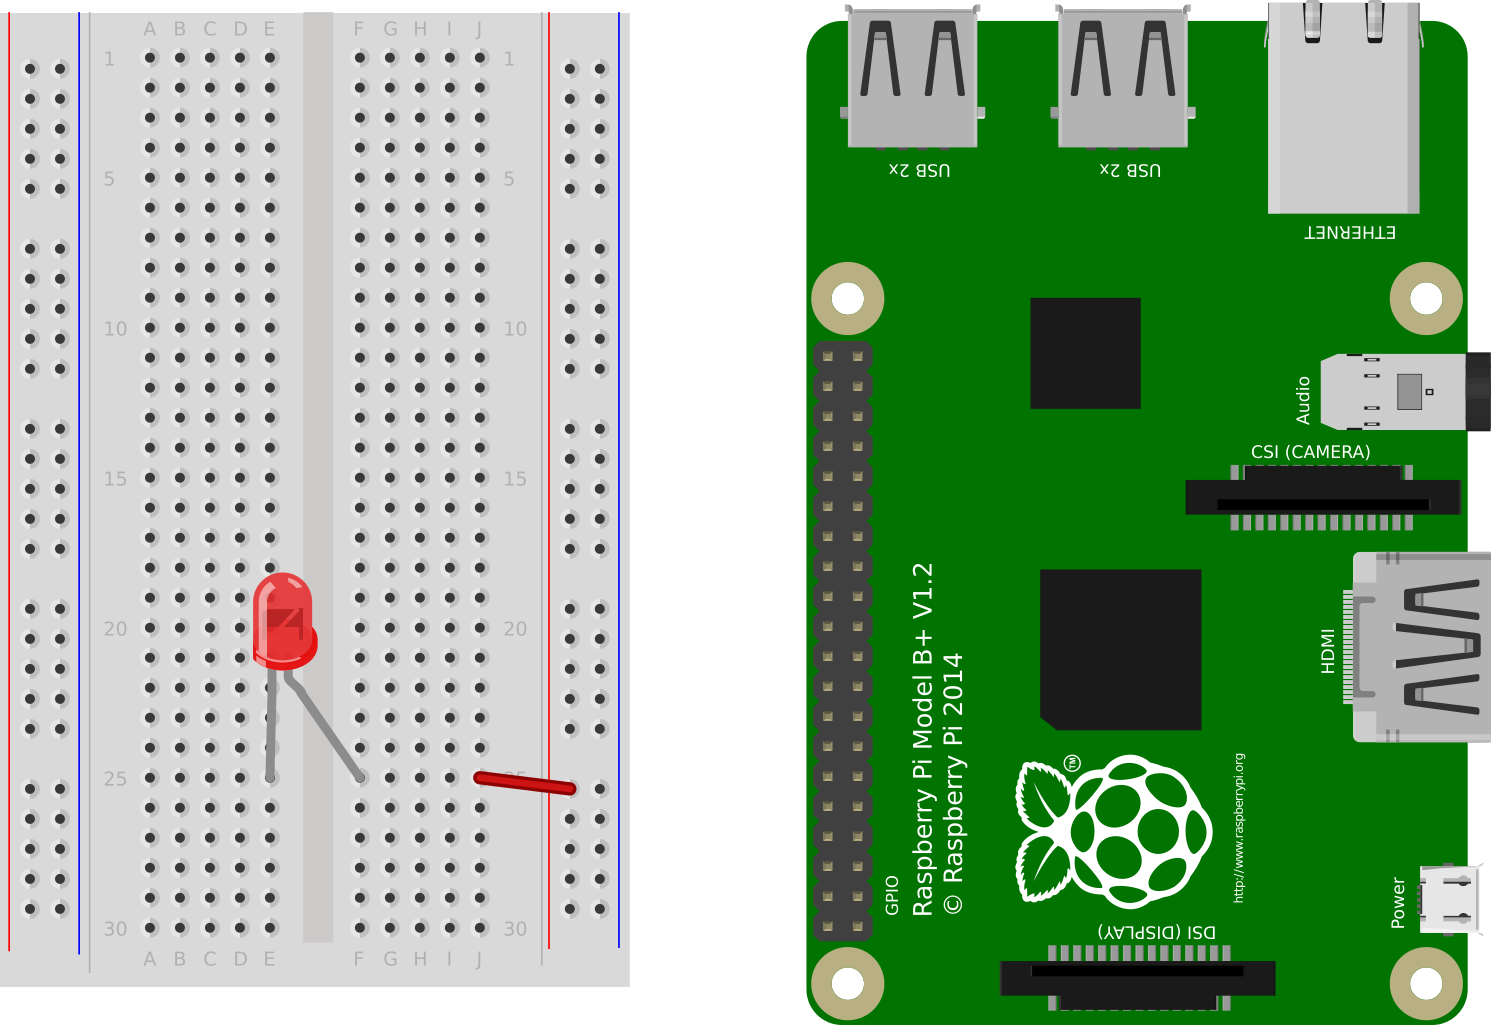
\includegraphics[width=0.7\linewidth]{McrRaspJam/015_GPIOZero/1_simplecircuit/2}
	\end{center}

	We then place a $68 \Omega$ resistor, connecting from the negative side of the LED to any other row, as shown.
	
	Then, connect the other end of the resistor to the negative power rail on the breadboard using another jumper cable.

	\begin{center}
		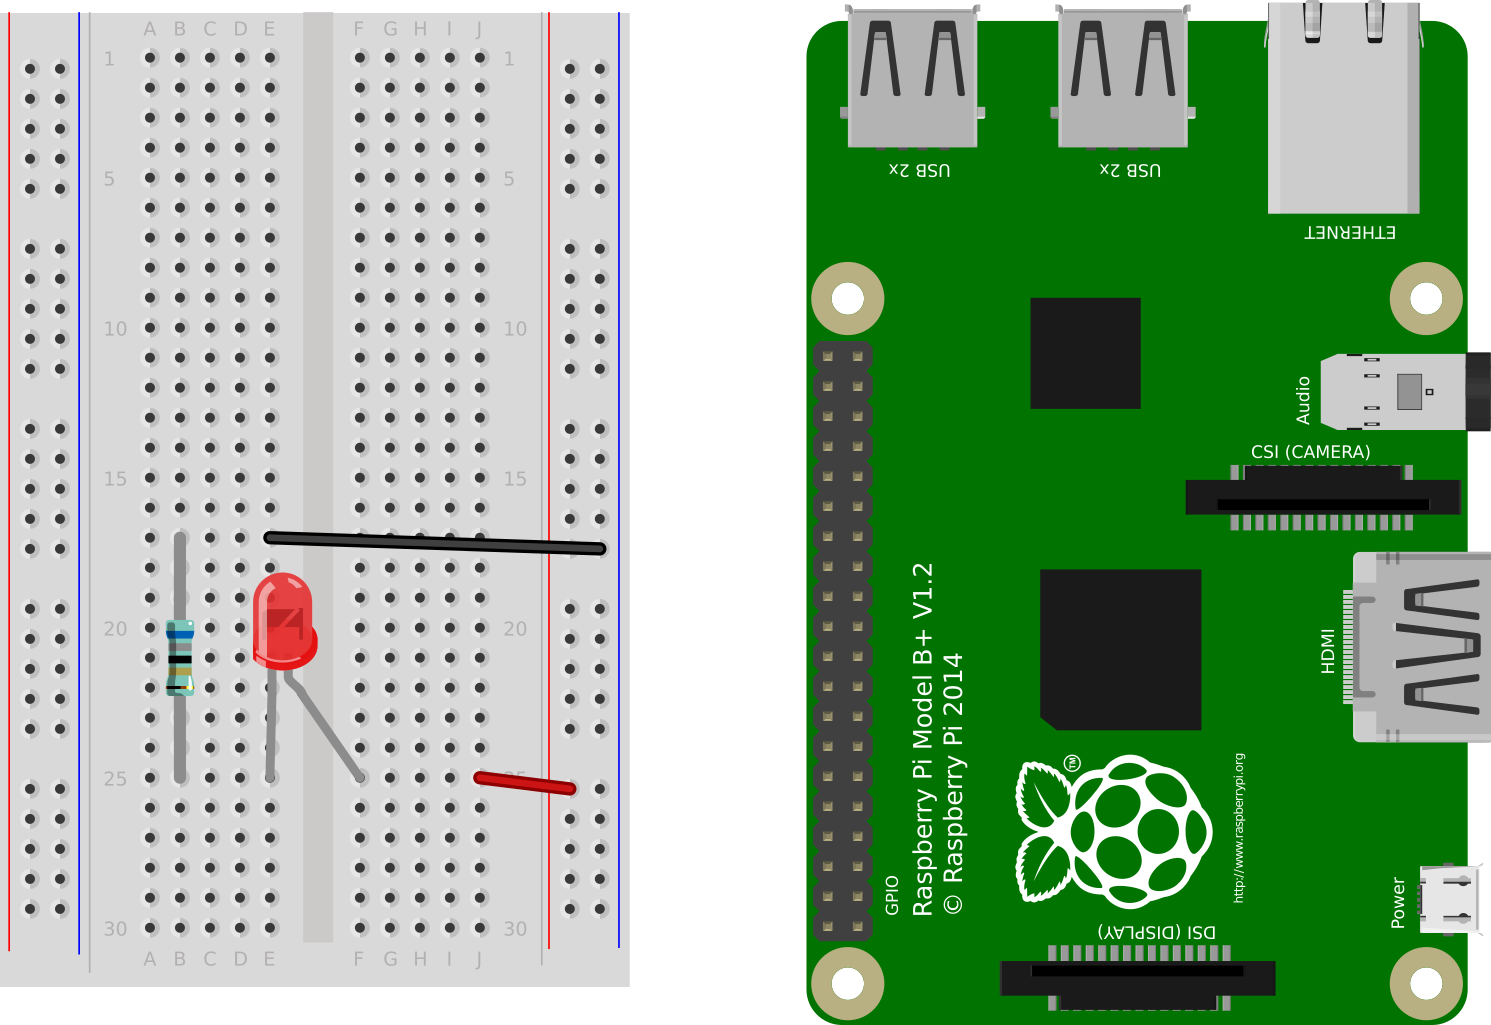
\includegraphics[width=0.7\linewidth]{McrRaspJam/015_GPIOZero/1_simplecircuit/4}
	\end{center}

	We've now created a full circuit from positive to negative. To power the circuit, we need to connect it to the power pins on our Raspberry Pi.
	
	Use a female-to-male jumper cable to connect the \textbf{positive} power rail on the breadboard to \textbf{3V3}, and the \textbf{negative} rail to \textbf{GND}.

	\begin{center}
		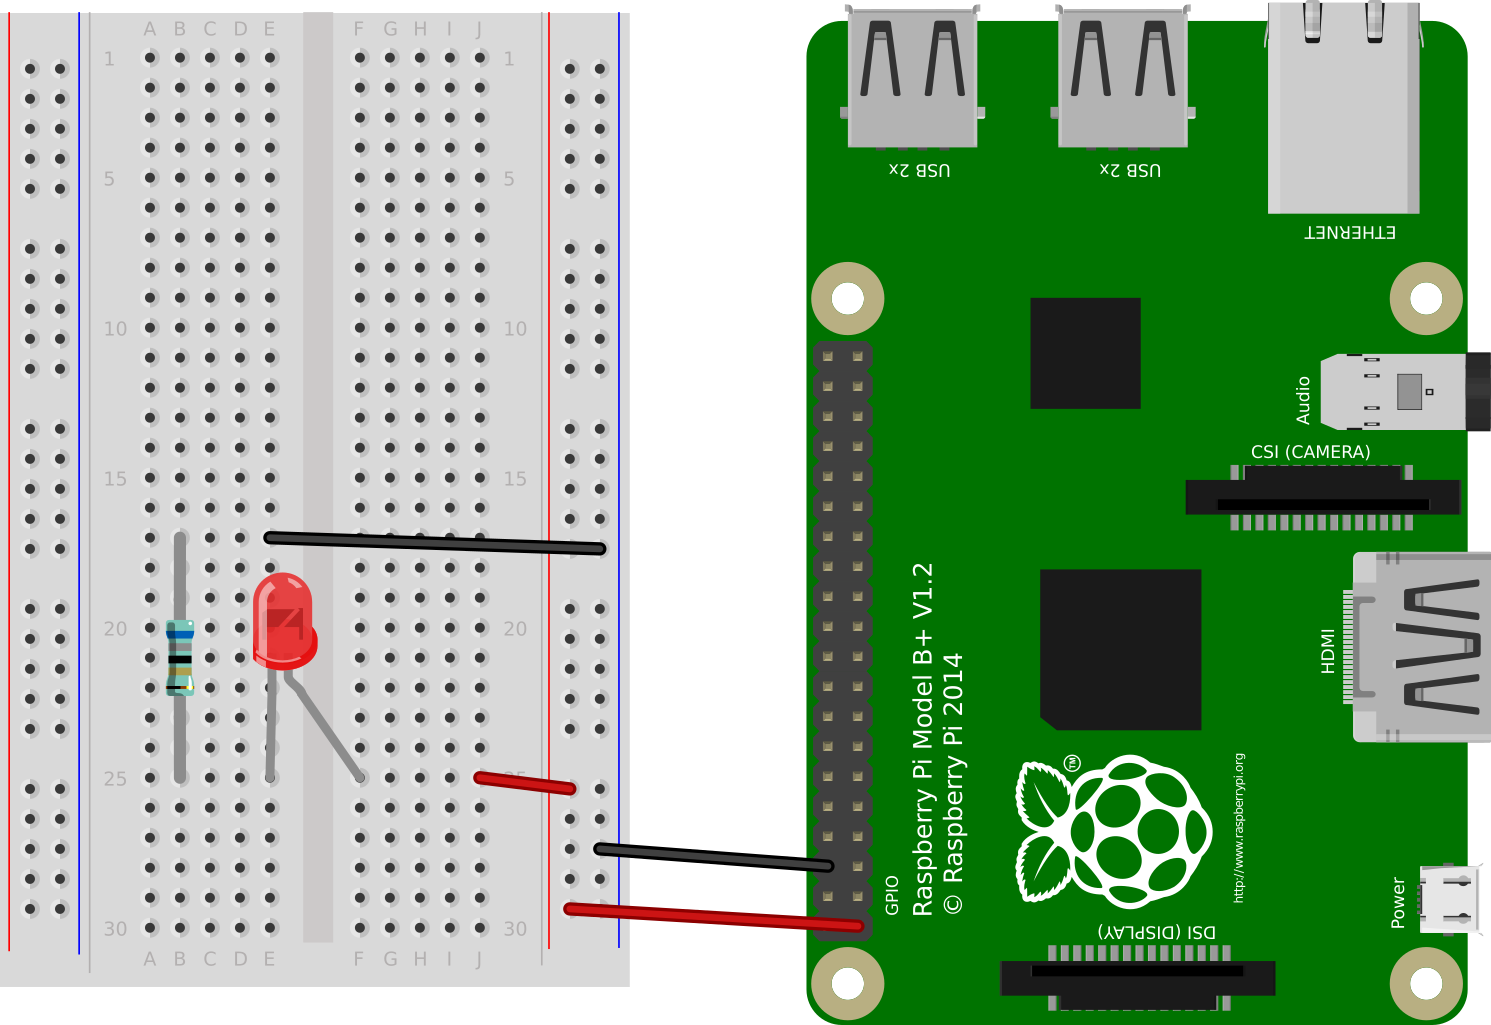
\includegraphics[width=0.7\linewidth]{McrRaspJam/015_GPIOZero/1_simplecircuit/5}
	\end{center}

	If all the connections are correct, your LED should light up.
	
	\subsection*{Our Circuit}
	
		We've just created a simple circuit that powers a single LED. If you've been taught circuit schematics before, the circuit we just built might look like this:
		
		\begin{center}
			
\includegraphics[width=0.5\linewidth]{McrRaspJam/015_GPIOZero/1_simplecircuit/schematic}
		\end{center}
		
		Right now our Raspberry Pi computer isn't controlling the LED, we're simply using the power supply to light the LED; this means our Raspberry Pi is currently just a \$35 battery.
		
		In order to control the LED, we'll need to alter the circuit to use GPIO pins.
		
		\subsection{Creating a GPIO circuit}
		
		Altering the circuit is straightforward. We will use one of the GPIO pins as an \textit{output}, meaning it will supply the power to the LED.
		
		Remove the jumper cables connecting to the positive power rail of the breadboard, and place a single female-to-male connecting the LED to a GPIO pin, as shown.
		
		\begin{center}
			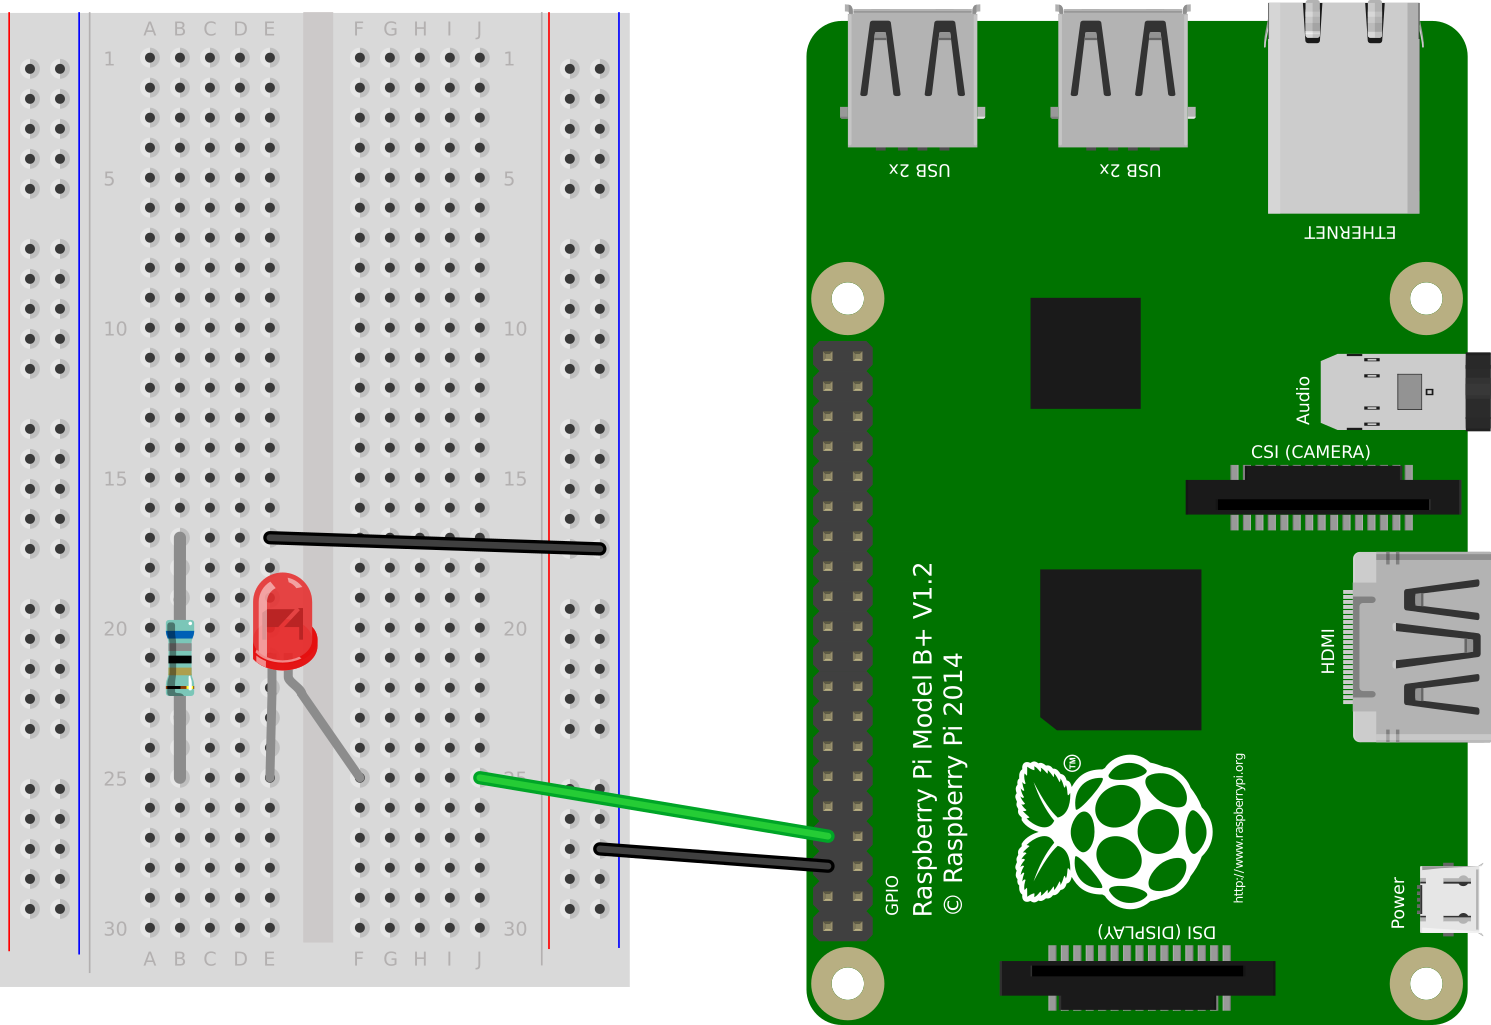
\includegraphics[width=0.7\linewidth]{McrRaspJam/015_GPIOZero/1_simplecircuit/6}
		\end{center}
	
		\subsubsection{Programming the LED}
		
			Now we have a simple GPIO circuit, we can have a go at programming our LED.
			
			Boot to the Raspbian desktop if you haven't yet done so, and from the application menu open \textbf{IDLE 3}. Click \mbox{\texttt{File → Open...}} and open \texttt{1\_led.py}.
			
			\lstinputlisting[style=Python, title=1\_led.py]{McrRaspJam/015_GPIOZero/1_simplecircuit/1_template.py}
			
			This program doesn't yet do anything, but it has loaded \textit{GPIO Zero} for us to use.
			
			First, we start by defining our LED. Make a note of the GPIO number you connected your LED to, (we used GPIO14) and enter the following line, substituting the pin number you connected:
			
			\lstinputlisting[style=Python, firstline=3, firstnumber=3, lastline=4]{McrRaspJam/015_GPIOZero/1_simplecircuit/1_led.py}
			
			Then use the \textit{function} \texttt{on()} to turn on your LED:
			
			\lstinputlisting[style=Python, firstline=5, firstnumber=5]{McrRaspJam/015_GPIOZero/1_simplecircuit/1_ledon.py}
			
			Now try running your program using \mbox{\texttt{Run → Run Module}}. When your program starts running your LED should turn on.
			
			Let's make our program a little more interesting by making our LED blink. We'll start by doing this the manual way, using a loop. Alter your program so it looks as follows.
			
			\lstinputlisting[style=Python]{McrRaspJam/015_GPIOZero/1_simplecircuit/1_led.py}
			
			Run your program again, and the LED should start blinking.
			
			How can you alter the program to make the blinking twice as fast? how about making it blink so that the light is on for 2 seconds and off for 1?
			
			That's not all though. GPIO Zero has lots of useful functions for each type of device. For LEDs, a function called \texttt{blink()} is provided to make it easy to blink an LED. We can replace our loop with a single line:
			
			\lstinputlisting[style=Python, firstline=4, firstnumber=4]{McrRaspJam/015_GPIOZero/1_simplecircuit/1_ledblink.py}
			
			\begin{aside}[GPIO Zero functions]
				GPIO Zero supports a lot of different devices, and each device has a number of useful functions for you to use.
				
				The easiest way to see them all is in the online documentation, which can be found at \href{https://gpiozero.readthedocs.io/}{\texttt{gpiozero.readthedocs.io}}
			\end{aside}
			